%!TEX root = ../main.tex

\chapter{Aktivität}
\label{chap:activity}

In Abbildung~\ref{fig:tasks} ist die Verteilung der Aufgaben unter unseren Teammitgliedern zu sehen.
Wie zu erkennen ist, wurde mit einzelnen Ausnahmen jedem Teammitglied für jede Woche eine Aufgabe zugeteilt.
Da wir vermuteten, dass die Umsetzung der Öffnungszeitenfunktion überdurchschnittlich kompliziert sein könnte,
entschieden wir uns, dieser Funktion zwei Wochen zuzuweisen.

Die im Diagramm dargestellte Zeitaufteilung wurde nahezu vollständig eingehalten,
die Zeitschätzungen bei der Aufteilung der Funktionen scheint dem tatsächlichen Aufwand also sehr nahe gewesen zu sein.

\begin{figure}[ht]
    \centering
    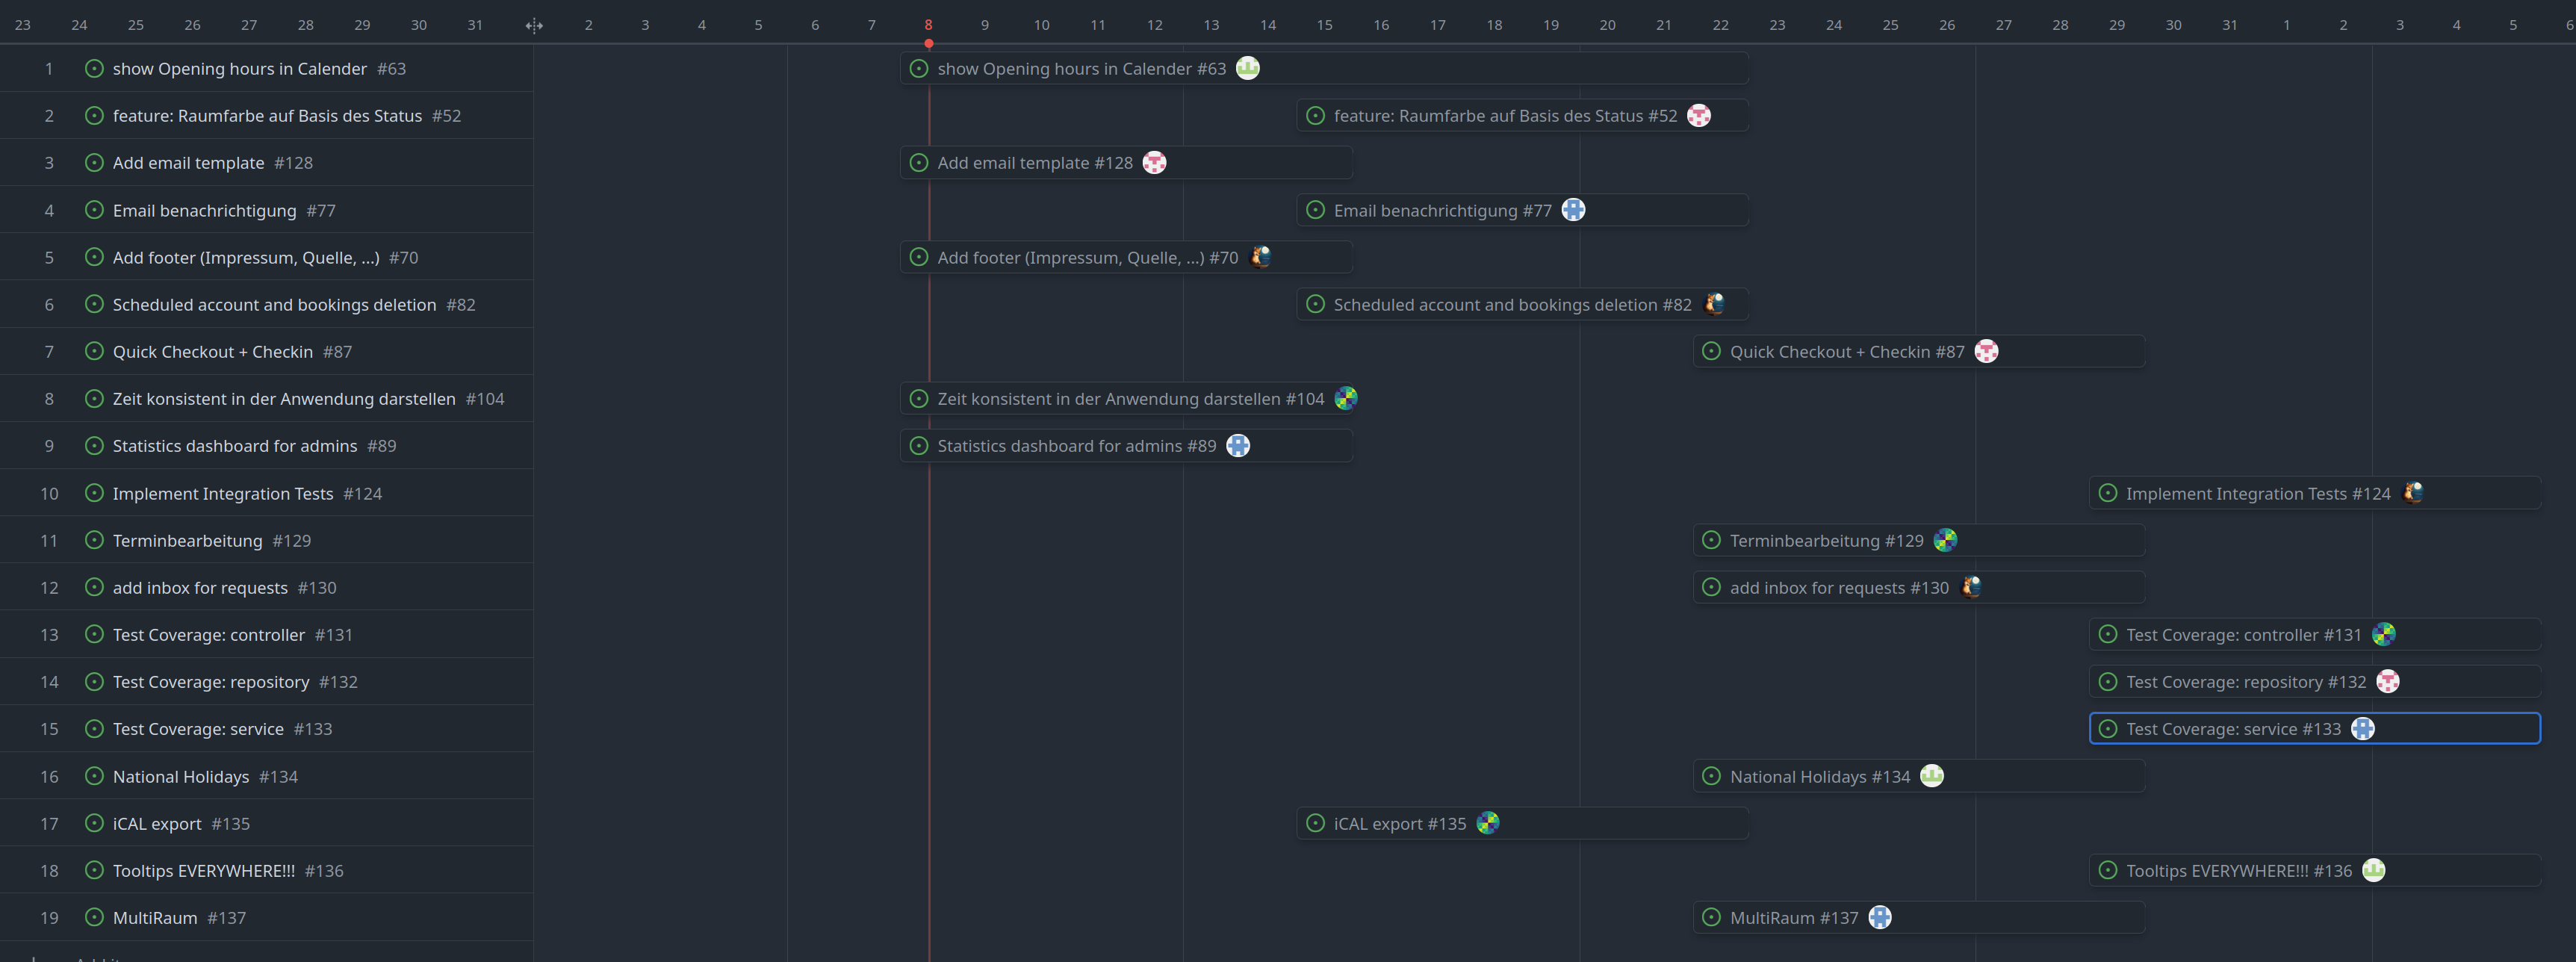
\includegraphics[width=\textwidth]{figures/tasks}
    \caption{Verteilung der Aufgaben}
    \label{fig:tasks}
\end{figure}

In Abbildung~\ref{fig:commits} ist die Verteilung der Commits pro Stunde und Wochentag dargestellt.
In dieser ist zu erkennen, dass die Entwicklung der Anwendung größtenteils in den üblichen Arbeitszeiten von 9 bis 17 Uhr verlief.
Während an Wochenenden und Feiertagen einzelne Commits vorkommen, sind diese in der Regel auf kleinere Änderungen beschränkt.
Für die Planung des Projekts ist dies ein klarer Erfolg, da die Aufgaben offenbar gut über die Zeit verteilt werden konnten.

\begin{figure}[ht]
    \centering
    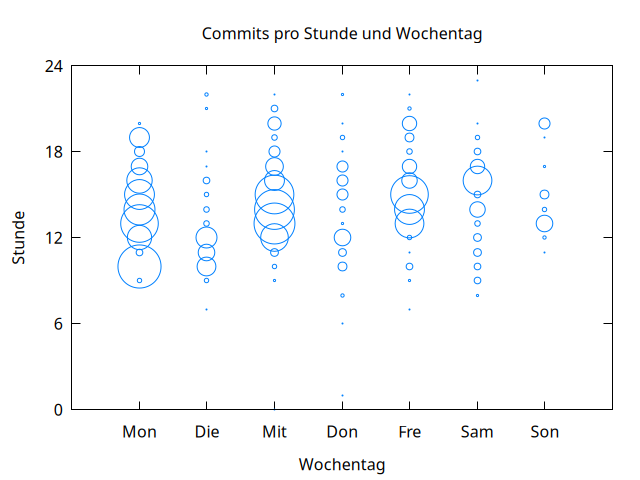
\includegraphics[width=\textwidth]{figures/hours}
    \caption{Commits pro Stunde und Wochentag}
    \label{fig:commits}
\end{figure}